\documentclass{article}

% if you need to pass options to natbib, use, e.g.:
\PassOptionsToPackage{numbers, sort&compress}{natbib}
% before loading neurips_2026

% The authors should use one of these tracks.
% Before accepting by the NeurIPS conference, select one of the options below.
% 0. "default" for submission
\usepackage[main,final]{neurips_2026}
% the "default" option is equal to the "main" option, which is used for the Main Track with double-blind reviewing.
% 1. "main" option is used for the Main Track
%  \usepackage[main]{neurips_2026}
% 2. "position" option is used for the Position Paper Track
%  \usepackage[position]{neurips_2026}
% 3. "eandd" option is used for the Evaluations & Datasets Track
 % \usepackage[eandd]{neurips_2026}
% 4. "creativeai" option is used for the Creative AI Track
%  \usepackage[creativeai]{neurips_2026}
% 5. "sglblindworkshop" option is used for the Workshop with single-blind reviewing
 % \usepackage[sglblindworkshop]{neurips_2026}
% 6. "dblblindworkshop" option is used for the Workshop with double-blind reviewing
 % \usepackage[dblblindworkshop]{neurips_2026}
% 7. "education" option is used for the Education Track
 % \usepackage[education]{neurips_2026}


% After being accepted, the authors should add "final" behind the track to compile a camera-ready version.
% 1. Main Track
 % \usepackage[main, final]{neurips_2026}
% 2. Position Paper Track
% \usepackage[position, final]{neurips_2026}
% 3. Evaluations & Datasets Track
 % \usepackage[eandd, final]{neurips_2026}
% 4. Creative AI Track
% \usepackage[creativeai, final]{neurips_2026}
% 5. Workshop with single-blind reviewing
% \usepackage[sglblindworkshop, final]{neurips_2026}
% 6. Workshop with double-blind reviewing
% \usepackage[dblblindworkshop, final]{neurips_2026}
% Note. For the workshop paper template, both \title{} and \workshoptitle{} are required, with the former indicating the paper title shown in the title and the latter indicating the workshop title displayed in the footnote.
% For workshops (5., 6.), the authors should add the name of the workshop, "\workshoptitle" command is used to set the workshop title.
% \workshoptitle{WORKSHOP TITLE}
% 7. Education Track
% \usepackage[education, final]{neurips_2026}

% "preprint" option is used for arXiv or other preprint submissions
 % \usepackage[preprint]{neurips_2026}

% to avoid loading the natbib package, add option nonatbib:
%    \usepackage[nonatbib]{neurips_2026}

\usepackage[utf8]{inputenc} % allow utf-8 input
\usepackage[T1]{fontenc}    % use 8-bit T1 fonts
\usepackage{hyperref}       % hyperlinks
\usepackage{placeins}
\usepackage{graphicx}       % figures
\usepackage{float}          % [H] tables stay with their text
\usepackage{url}            % simple URL typesetting
\usepackage{booktabs}       % professional-quality tables
\usepackage{amsfonts}       % blackboard math symbols
\usepackage{amsmath}        % math environments
\usepackage{amssymb}        % math symbols
\usepackage{nicefrac}       % compact symbols for 1/2, etc.
\usepackage{microtype}      % microtypography
\usepackage{xcolor}         % colors
\usepackage{textcomp}       % cent sign in the reward table

% Section numbers carry a trailing dot in the heading (cross-references unchanged).
\makeatletter
\renewcommand{\@seccntformat}[1]{\csname the#1\endcsname.\quad}
\makeatother

% Note. For the workshop paper template, both \title{} and \workshoptitle{} are required, with the former indicating the paper title shown in the title and the latter indicating the workshop title displayed in the footnote.
\title{One Shared PPO Policy for Heterogeneous Commercial Building HVAC Control}


% The \author macro works with any number of authors. There are two commands
% used to separate the names and addresses of multiple authors: \And and \AND.
%
% Using \And between authors leaves it to LaTeX to determine where to break the
% lines. Using \AND forces a line break at that point. So, if LaTeX puts 3 of 4
% authors names on the first line, and the last on the second line, try using
% \AND instead of \And before the third author name.


\author{%
  Sidharthan S \\
  Independent Researcher \\
  \texttt{sid250581@gmail.com} \\
  % examples of more authors
  % \And
  % Coauthor \\
  % Affiliation \\
  % Address \\
  % \texttt{email} \\
  % \AND
  % Coauthor \\
  % Affiliation \\
  % Address \\
  % \texttt{email} \\
  % \And
  % Coauthor \\
  % Affiliation \\
  % Address \\
  % \texttt{email} \\
  % \And
  % Coauthor \\
  % Affiliation \\
  % Address \\
  % \texttt{email} \\
}


\raggedbottom

\begin{document}
\nocite{goldfeder2024smart,goldfeder2026smart}


\maketitle


\begin{abstract}
Heating, ventilation, and air-conditioning (HVAC) systems govern indoor environmental quality in modern buildings, operating under the dual imperative of minimizing energy consumption while strictly preserving occupant thermal comfort. However, simultaneously satisfying these objectives remains challenging due to complex building thermal dynamics, fluctuating weather, and stochastic occupancy patterns, which differ from one building to the next. In this work, we show that a single shared Proximal Policy Optimization (PPO) policy, trained solely on the joint 3C (comfort, cost, and carbon) reward, achieves robust zero-shot generalization across disparate building environments. Specifically, trained across 30 scenarios spanning six distinct building layouts and five climate zones, the policy scores 0.0165 against 0.0461 for the benchmark's PID controller on 90 held-out months, and holds in a completely unseen Minneapolis climate. Furthermore, our findings remain validated entirely within the benchmark's simulator, leaving sim-to-real transfer to future physical testbed deployments. More broadly, the result suggests that a heterogeneous stock is as much a problem of representation as of control: one fixed layout let a single policy cover buildings from 30 to 85 zones without per-building training.
\end{abstract}


\section{Introduction}

\textbf{Context}: Achieving global decarbonization depends heavily on reducing the environmental footprint of the built environment. According to the United Nations Environment Programme \citep{unep2025buildings} and the International Energy Agency \citep{iea2018futureofcooling}, the buildings and construction sector accounts for 34\% of global energy and process $\text{CO}_2$ emissions. Rather than declining in line with climate targets, sector-wide operational emissions rose from 9.3 $\text{GtCO}_2$ in 2015 to a record 9.8 $\text{GtCO}_2$ in 2023, representing a 5.4\% increase. Commercial (non-residential) buildings alone contribute 10\% of total global emissions \citep{eia2018cbecs}, which constitutes roughly 29.4\% of all building-sector emissions. The operational footprint of these facilities is driven primarily by heating, ventilation, and air-conditioning (HVAC) systems.

\textbf{Building control:} A building's HVAC infrastructure consists of interconnected thermal zones served by a central network of heating, cooling, and air-distribution equipment. A central plant supplies heated and chilled water to air-handling units (AHUs), which condition and distribute air through duct networks, while variable air volume (VAV) boxes regulate the airflow delivered to individual zones through dampers and local reheat coils. A building controller monitors measurements from the zones and central plant and acts at both levels: it sets the plant and air-handler operating points, such as hot-water loop temperature and supply-air temperature, and it positions the zone dampers and reheat valves. Rather than directly setting individual zone temperatures, these commands influence the thermal environment indirectly through the building's HVAC equipment and physical dynamics.

\textbf{Challenges in Smart Building Control:} Controlling HVAC systems in commercial buildings presents several interconnected challenges. \textbf{First}, buildings exhibit substantial thermal inertia: structural mass, floors, and furnishings absorb and release heat gradually, causing the thermal impact of a setpoint adjustment to become apparent only after a significant delay. \textbf{Second}, occupancy decides where the objective is charged. As occupants arrive and depart, thermal and ventilation demand shifts across zones, and the score bills comfort only in occupied zones while it bills energy and carbon at every step. A controller has to hold the band where people are, let the empty zones drift, and it sees only a building-wide occupant count rather than which zone is occupied. \textbf{Third}, the operating point that is efficient depends on the weather outside. The same building needs different supply-water and supply-air temperatures in a cold month and a warm one, so a controller that covers both has to move its operating point with the weather rather than hold one setting. To investigate these challenges, the \textbf{Smart Buildings Control Suite} \citep{goldfeder2024smart} provides a standardized environment comprising measured building data, building-specific calibrated simulation environments, and a common control interface.

\textbf{Key contribution:} We design a shared control architecture that enables standard Proximal Policy Optimization (PPO; \citep{schulman2017proximal}) to operate across heterogeneous building configurations. Implemented within the high-throughput \textbf{PufferLib} framework, our approach uses a single shared policy to control buildings with varying numbers of thermal zones and air-handling units, rather than relying on independently trained controllers. We achieve this through a common slot-based representation with equipment-existence indicators, allowing the policy to accommodate variable building configurations using shared parameters. To address the delayed dynamics of HVAC systems, we incorporate historical thermal information, projected comfort deficits, and airflow-related features into the policy's observations. We also employ bounded Beta action distributions to produce valid control commands at every step. Across all training scenarios, the policy directly optimizes the benchmark's joint 3C objective, balancing thermal comfort, operational cost, and carbon emissions without facility-specific reward tuning.

\section{Related Works}

\textbf{Benchmark:} Reinforcement learning has been applied to HVAC control from individual thermal zones to whole-building energy management \citep{wei2017deep,yu2021review}, and a notable real deployment reports 9\% and 13\% energy savings across two commercial facilities \citep{luo2022controlling}. Interacting with buildings is costly, and model-predictive control needs a calibrated model of every building \citep{afram2014theory}, so the Smart Buildings Control Suite trains agents in calibrated simulators built from real telemetry \citep{blum2019prototyping,goldfeder2024smart}. The Smart Buildings Challenge then adds procedurally generated buildings and held-out configurations, to ask whether a learned controller transfers across unseen buildings and climates \citep{goldfeder2026smart}.

\textbf{Offline and online reinforcement learning:} HVAC control studies differ in how agents acquire their experience. Offline reinforcement learning learns from previously collected logs, which avoids exploration and cannot test alternatives the logs never contain \citep{blad2022data,levine2020offline}. Simulation-based training provides a safer setting for exploring alternative control strategies, while recent studies have also investigated transferring simulation-trained policies to real buildings through online adaptation \citep{coraci2023online}. In this work, we adopt interactive simulation-based PPO training, allowing the policy to learn from newly generated environment experiences rather than relying exclusively on fixed historical trajectories.

\textbf{Scalability and generalization across buildings:} Transfer learning reuses a controller trained on source buildings: cross-building transfer of pretrained DQN controllers \citep{fang2023cross}, multi-source transfer for multi-zone control \citep{hou2024multi}, heterogeneous transfer across buildings with different energy systems and state representations \citep{coraci2024heterogeneous}. Each adapts a pretrained controller to a target building; we instead train one shared policy across heterogeneous buildings at once, without target-specific fine-tuning.

\section{Methods}

\subsection{Problem formulation and control environment}

We formulate building climate control as a discrete-time \textbf{partially observed Markov decision process (POMDP)}, $(\mathcal{S}, \mathcal{A}, \mathcal{T}, \mathcal{R}, \Omega, \mathcal{O}, \gamma)$ \citep{garcia2013mdp,sutton2018reinforcement}. Table~\ref{tab:interface} gives the observation, the hybrid action space and the reward.

\begin{table}[h]
\centering
\small
\renewcommand{\arraystretch}{1.35}
\begin{tabular}{@{}p{0.21\linewidth}p{0.73\linewidth}@{}}
\toprule
Space / representation & Parameters and ranges \\
\midrule
\textbf{Observation ($o_t$)} & Flat float32 vector of building-dependent length ($d$): zone temperatures, heating/cooling setpoints, flows, damper and reheat echoes, AHU supply/static states, loop temperatures and pressures; 16 of the 48 supplied diurnal and weekly harmonics; two comfort flags; building-wide occupancy, $(n-125)/126$. \\
\addlinespace[3pt]
\textbf{Action ($a_t$)} & $a^{\text{cont}}\in[-1,1]^{3K+2V+2}$, $a^{\text{disc}}\in\{0,1\}^{K+1}$. Supply air 285--305 K; supply water 310--350 K; static pressure 0--2000 Pa; loop differential pressure 0--20; damper, reheat and recirculation $[0,1]$; on/off for the $K$ handlers and the pump. \\
\addlinespace[3pt]
\textbf{Reward ($r_t$)} & Comfort $C_1$ (occupancy-weighted productivity, \$300 per occupant-hour), energy cost $C_2$ (hourly electricity price of 16--20\,\textcent/kWh plus a monthly gas price) and carbon emission $C_3$ (hourly grid intensity of 87.8--104.7\,g/kWh plus a constant gas rate); all non-positive, unclipped, and zero at the ideal. \\
\addlinespace[3pt]
\textbf{Horizon} & $\Delta t=300$ s; $T=8{,}640$ steps (30 days); discounted training return with $(\gamma,\lambda)=(0.99,0.95)$; evaluation is the negated undiscounted mean per-step reward, averaged across scenarios. \\
\bottomrule
\end{tabular}
\vspace{4pt}
\caption{The control interface of the benchmark environment.}
\label{tab:interface}
\end{table}

The dynamics are \textbf{deterministic} given the commands and the scenario's weather trace: thermal mass delays the response by minutes to hours. Randomness enters only through occupancy. The controller never sees the full state: the mass temperature inside each control volume, the occupancy of an individual zone (only a building-wide count is reported), and the building's identity, weather name or month (only diurnal and weekly harmonics are given). The policy recovers the missing per-zone and temporal context from history (\S3.3); Appendix~A gives the model and Appendix~B the input contract.

The policy acts \textbf{directly on the equipment}, without a rule-based sequence or safety filters. Whatever behaviour it shows is learned from interaction with the simulator.

{\samepage
Each step returns the benchmark's \textbf{3C reward} in the benchmark's notation,
\[
r_t = 0.6\,C_1 + 0.2\,C_2 + 0.2\,C_3,
\]
where $C_1 \le 0$ is the occupancy-weighted comfort term, scored against the standard thermal-comfort band of the benchmark \citep{ashrae55} (zero inside the band and whenever the building is empty, falling linearly over the first 5 K outside it and quadratically beyond), $C_2 \le 0$ the energy cost and $C_3 \le 0$ the carbon emission. No term is clipped, and the objective is unmodified: no shaping, potential or extra comfort term.
}

% NOTE (content.md, not paper prose): What to move to the appendix so this stays a subsection: the arity formula in words, field ordering and the `_1` collision convention, missing-value fill, the full state enumeration, the exact normalisation denominators, the per-op float32 decode identity, and the two-level score definition with its equation. None of them are needed to follow \S3.2--\S3.5, and all are needed by someone re-implementing you.
% NOTE (content.md, not paper prose): One judgement call worth making deliberately: keep the ``no building identifier'' clause in \S3.1 rather than in \S3.5. It reads there as a property of the interface, not as a defence of a claim, and it is the sentence that makes your generalization result about the policy instead of about the data.

\subsection{GPU-Accelerated Simulation Infrastructure}

To enable large-scale parallel training, we port the complete building simulation environment to CUDA, integrating the environment with PufferLib's vector interface \citep{suarez2024pufferlib} and CUDA graph execution. The port is validated against the reference Python implementation. With double-precision physics, the implementation sustains 12K environment steps per second (SPS) on an NVIDIA L40S and 6.2K SPS on an RTX 3090, while the reference Python simulator reaches about 145 SPS on 12 CPU cores. Implementation details, validation and throughput are in Appendix~A.

\subsection{Shared Policy Architecture and Observation Design}

One policy must control buildings of different size with a single set of weights. We achieve that with two choices: an interface identical for every building, and readouts shared by equipment role rather than by zone.

Buildings differ in their numbers of zones and air handlers, so their raw observations are structurally incompatible. We map every building into the same 983-value vector: 90 zone slots, 9 air-handler slots, one hot-water slot and one global slot. Absent slots are zero, device fields are returned to physical units with the constants the gateway supplies, and each group is put on a fixed scale, so the same slot means the same thing in every building (Figure~\ref{fig:arch}; Appendix~B).
% NOTE: panel (b) of the figure is the padded 90-slot layout (the 54-zone building, 36 of 90
% slots zero). Whether that padding detail is main-text or appendix is still open, so the prose
% pointer to panel (b) is removed for now; restore it if the padding case stays in the main text.

\begin{figure}[h]
\centering
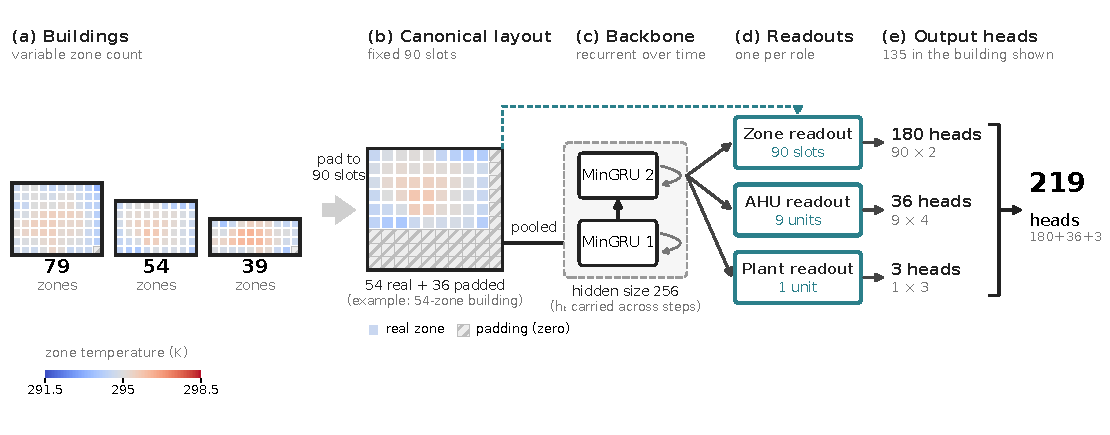
\includegraphics[width=\linewidth]{figures/fig_architecture_v2.pdf}
\caption{Architecture of the shared control policy. (a) Training buildings (79, 54, and 39 zones), zones shaded illustratively by temperature on a shared scale. (b) State slotization: buildings map into 90 fixed zone slots (e.g., 54 active zones and 36 zero-padded slots), 9 AHU slots, 1 plant slot and 1 global slot, 983 values in all. (c) An 80-value pooled summary enters a two-layer recurrent backbone (256 hidden units per layer) that carries one state across steps; each readout also reads its own local slice, 68 values for a zone, 32 for an air handler and 16 for the plant. (d) Shared readout networks grouped by equipment role rather than individual identity. (e) Multi-head policy: 219 heads, 180 for zones (damper and reheat), 36 for AHUs (supply temperature, static pressure, recirculation, on/off) and 3 for the central plant; the pictured building uses 135, and a head a building does not have is masked.}
\label{fig:arch}
\end{figure}

An 80-value pooled summary of that vector (zone and air-handler statistics, plant state, equipment presence, time and occupancy) enters two minimal-GRU layers of 256 hidden units \citep{feng2024rnn}, so the building carries one recurrent state across steps that every slot reads. Each slot's readout combines that state with role-specific local features. For a zone these are its own seven values (temperature, the two setpoint deficits, the heating setpoint, the damper and reheat echoes and presence), the rectified part of each deficit, the eight sensor and echo values of its air handler, and the four sibling entries of every slot in its group, its own included, so a zone is conditioned on its neighbours without a learned attention layer; with the eleven delay features below, a zone reads 68 values, an air handler 32 and the plant 16. Air-handler slots read their own eight values and statistics aggregated over their zones, plus the plant's two loop values. Zone slots also carry a four-hour ring (48 steps) of their own temperature and comfort deficit, from which the history features of Appendix~C are computed.

One readout is shared by every slot of the same role (zone, air handler, plant) rather than learned per zone \citep{zaheer2017deepsets}, so the whole network is 453K parameters shared by all 30 training scenarios. Each zone readout adds a shared 32-unit tanh branch with a zero-initialised output, so at initialisation every head is a fixed affine function of the state and only the nonlinear correction has to be learned. The slot layout has 219 heads; a building masks the ones it does not have and commands between 75 and 209 of them. The critic reads the same trunk state and no input the actor does not see, and it is a state baseline rather than an action-dependent one \citep{tucker2018mirage}. One parameter set therefore serves every zone, air handler and plant in every building.

\subsection{Bounded Action Parameterisation and Policy Optimisation}

\subsubsection{Admissible Control via Bounded Beta Distributions}

To control continuous physical actuators without post-hoc clipping or boundary artefacts, each active head outputs a bounded Beta distribution rather than a standard Gaussian. The policy runs on a padded interface of 256 continuous and 16 discrete heads. It uses 219 continuous heads and no discrete head; a building masks every head it does not have. Rather than squashing an unbounded Gaussian with a $\tanh$ function, which saturates gradients near the limits, or applying an external projection, each head models a Beta distribution over $(0,1)$ \citep{chou2017beta} and emits
\[
a = 2x - 1, \qquad x \sim \operatorname{Beta}(\alpha, \beta);
\]
$a$ is mapped affinely to the range of a continuous command, and the ten on/off commands are read as on when $a > -0.5$.
We compute the shape parameters from the network outputs $u$ and $v$ as
\[
\alpha = \operatorname{softplus}(u) + 0.5, \qquad \beta = \operatorname{softplus}(v) + 0.5.
\]
The $0.5$ floor lets the density form a central mode ($\alpha,\beta>1$) or a bimodal U-shape ($\alpha,\beta<1$), so a damper can be held firmly open or shut; Appendix~H measures which shape the reported policy uses for each actuator. To prevent entropy from vanishing during training, we cap the sum $\alpha+\beta$ at 12: whenever it would exceed 12, both parameters are rescaled by $12/(\alpha+\beta)$, which preserves the mean $\alpha/(\alpha+\beta)$ while bounding policy certainty. Because every sample is natively bounded, all emitted actions are admissible by construction: no external filtering, clipping or projection sits between the policy and the plant (Appendix~D).

\subsubsection{Multi-Head PPO and Horizon Scaling}

Optimising up to 209 actuators at once creates a failure mode for standard policy-gradient updates: a joint ratio lets large steps on a few heads hide behind near-zero shifts on the others. We remove this cross-head interference by decoupling the PPO clipping objective across individual control slots \citep{han2019dimension}. Each active head $h$ keeps its own importance ratio at the stored sample,
\[
r_h(\theta) = \frac{\pi_\theta(x_h \mid s)}{\pi_{\theta_{\mathrm{old}}}(x_h \mid s)}.
\]
Each ratio is clipped independently to $[0.8, 1.2]$, that is $\epsilon = 0.2$, and the surrogate sums these clipped objectives over the building's active heads, $\mathcal{H}$,
\[
\mathcal{L}^{\mathrm{CLIP}}(\theta) = \hat{\mathbb{E}}_t\left[\,\sum_{h\in\mathcal{H}} \min\left(r_{h,t}(\theta)\hat{A}_t,\ \operatorname{clip}\left(r_{h,t}(\theta),\, 1-\epsilon,\, 1+\epsilon\right)\hat{A}_t\right)\right].
\]
The clip keeps each head inside its trust region.

To stabilise learning across buildings with widely differing baseline returns, advantages are standardised over the entire rollout buffer. We set $\gamma = 0.99$ and $\lambda = 0.95$: the return discounts over $1/(1-\gamma) = 100$ steps, eight hours, while the advantage weights a reward $k$ steps back by $(\gamma\lambda)^k$, an effective credit-assignment horizon of about 17 steps \citep{schulman2016gae}, 1.4 hours. That horizon covers the hourly tariff step and the first part of the thermal response, so a price spike attributes credit to the decision that caused it. The policy updates with Adam under a global gradient-norm cap of 0.5, a value coefficient of 0.5, an entropy bonus of 0.001 and a single shared learning rate. We use no reward shaping, potential function or auxiliary objective: the optimisation gradient is the competition score.

\subsubsection{Occupancy-Weighted Zone Critics}

A building-level scalar reward cannot identify which room caused an environmental violation or wasted conditioned air. To direct credit to local actuators without training hundreds of separate networks, we decompose the global reward into per-zone streams,
\[
r_{z,t} = 0.6\,p_{z,t} - 0.2\,s_{z,t}E_t - 0.2\,s_{z,t}C_t, \qquad s_{z,t} = \frac{o_{z,t}}{\sum_{z'} o_{z',t}},
\]
where $p_{z,t}$ measures zone $z$'s local thermal productivity regret, and $E_t$ and $C_t$ are the building's total energy and carbon expenditures. Fuel and carbon costs are allocated to each zone by its share of building occupancy $s_{z,t}$. The allocation conserves on occupied steps: summing the zone streams gives the building-level reward, and an empty building reduces every zone stream to zero.

The critic mirrors this decomposition. Built on the pooled latent representation, the value network outputs one building-level evaluation and 90 parallel zone-level evaluations. The 90 zone predictions share a single value loss, averaged over batch steps and the 90 slots, and their advantages are computed by generalised advantage estimation (GAE). Each zone action head is therefore guided by a local, spatially accurate advantage, giving fine-grained credit across dozens of thermal zones while the network stays single and compact.

\subsection{Training configuration}

\textbf{Scenarios and parallel environments.} Training spans 30 scenarios: six building topologies crossed with five diverse climates (Atlanta, Denver, Fairbanks, Phoenix and Singapore). We run 32 parallel environments per scenario (960 total), collecting 288 steps per worker to yield 276,480 transitions per policy update. Episode starts are staggered per environment, and the scenarios carry different months.

\textbf{Objective, budget and precision.} Training optimises the raw 3C reward of Section 3.1 without modification. The reported policy starts from a fresh random initialisation (seed 75) and runs for 199,895,040 environment steps, 723 rollouts, with the learning rate annealed linearly from $10^{-4}$ to zero over that same budget, so the reported checkpoint is taken at zero step size rather than mid-drift. Adam \citep{kingma2015adam} updates minibatches of 2,304 with four epochs per rollout, the batch design of \citet{andrychowicz2020matters}. The reported run trains on the double-precision solve, as does every score in this paper. A single-precision solve exists as an opt-in speed experiment and is not used here: it moves the observation by about $1.2\times10^{-4}$ against the double-precision reference, ten orders of magnitude above the default path's $2\times10^{-14}$, which is enough to change the reward the policy is trained on (Appendix~A.4). One 46 GB NVIDIA L40S sustains about 12K environment steps per second, so the full run takes roughly 4.6 hours (Appendix~A.3 and Appendix~E).

\section{Results}

Four policies appear in every comparison. \textbf{PID} is the water-based controller the benchmark ships. \textbf{Long} is the earlier 30-scenario run: a 1.5B-step budget with no linear anneal, stopped at 507.6M steps, whose best save is at 89.6M. \textbf{Mid} and \textbf{Final} are two saves of the later 30-scenario run, which budgets 199.9M steps and anneals the learning rate linearly to zero over that budget with a simplified recipe. Mid is the 159.3M save; Final is the 199.1M save, the last complete one and the policy this paper reports. Appendix~E gives both recipes and the checkpoint selection; Appendix~F the metric, the baseline and the public split; Appendix~G the two sets, the 54-month extension and the fuel.

Two held-out sets are reported and never pooled. The first is 90 months: five buildings under 18 weather windows, with two buildings and the Minneapolis climate never trained. The second is a 54-month extension on the three shipped buildings missing from the first set, on the same 18 windows.

\subsection{The score, the terms and the two budgets}

\begin{table}[h!]
\centering
\small
\setlength{\tabcolsep}{4.0pt}
\begin{tabular}{@{}lrrrrrrr@{}}
\toprule
 & steps (M) & comfort & energy & carbon & 90 months & 54 months & public \\
\midrule
\texttt{PID} & -- & 0.0326 & 0.0078 & 0.0057 & 0.0461 & 0.0437 & 0.0640 \\
Long & 507.6 of 1500.2 & 0.0137 & 0.0059 & 0.0057 & 0.0253 & 0.0192 & 0.0182 \\
Mid & 199.9, annealed & 0.0080 & 0.0054 & 0.0051 & 0.0185 & 0.0112 & 0.0175 \\
Final & 199.9, annealed & \textbf{0.0070} & \textbf{0.0051} & \textbf{0.0044} & \textbf{0.0165} & \textbf{0.0098} & 0.0294 \\
\bottomrule
\end{tabular}
\vspace{4pt}
\caption{The four policies on the 90-month set, the 54-month extension and the public leaderboard. The three terms are those of the reward in Section~3.1 with its sign removed, so they sum to the 90-month score; zero is the ideal and lower is better.}
\label{tab:score}
\end{table}


Final scores 0.0165 on the 90 months, 64\% below PID's 0.0461, 35\% below Long's best save and 11\% below Mid, and it is lower than PID on 89 of the 90 months; the exception is \texttt{train\_3}/\texttt{fairbanks\_6}, 0.0459 against 0.0410. On the 54-month extension it is 0.0098, 78\% below PID, 49\% below Long and 13\% below Mid, lower on all 54. Mid takes the public leaderboard, 0.0175 against Final's 0.0294, Long's 0.0182 and PID's 0.0640: the public split (Appendix~F) prefers the mid-anneal save, while the 90 and 54 months and all five buildings prefer Final.


The score is the sum of three terms, and Final's gain is mostly comfort: 0.0070 against 0.0326 for PID, 0.0137 for Long and 0.0080 for Mid, while energy falls from 0.0078 to 0.0051 and carbon from 0.0057 to 0.0044. Comfort is the largest term and the largest fall in every comparison, so no term is bought with another (Table~\ref{tab:score}, Figure~\ref{fig:scores}a).

\begin{figure}[t]
\centering
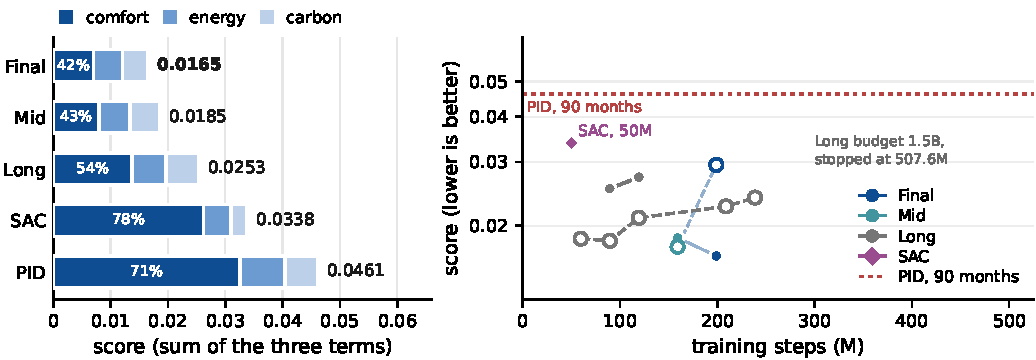
\includegraphics[width=\linewidth]{figures/fig_results_scores_v2.pdf}
\caption{The four policies. (a) The 90-month score as the sum of its three terms, printed at the bar end; comfort is the largest term in every bar. (b) Score against training steps on the 90 months (filled, solid) and on the public leaderboard (open, dashed). Long is best at 89.6M on both and its public score rises afterwards; the later run improves to 199.1M on the 90 months, while its public score is best at 159.3M. The dotted line is \texttt{PID} on the 90 months, comparable only to the filled series.}
\label{fig:scores}
\end{figure}

\FloatBarrier

\subsection{By building and by climate}

Final is below each of the other three on every building and every climate. Its building scores run from 0.0078 on \texttt{train\_2} to 0.0443 on \texttt{train\_3}, below Mid's 0.0087--0.0486, Long's 0.0132--0.0497 and PID's 0.0354--0.0689; its climate scores from 0.0112 in Phoenix to 0.0184 in Fairbanks, below the other three on all six. The two buildings never trained behave like the rest: on \texttt{train\_6} Final is 0.0126 against PID's 0.0491, and on \texttt{train\_3} 0.0443 against 0.0689; the 40 months of the unseen Minneapolis climate are 0.0180 against 0.0519.

\begin{figure}[h]
\centering
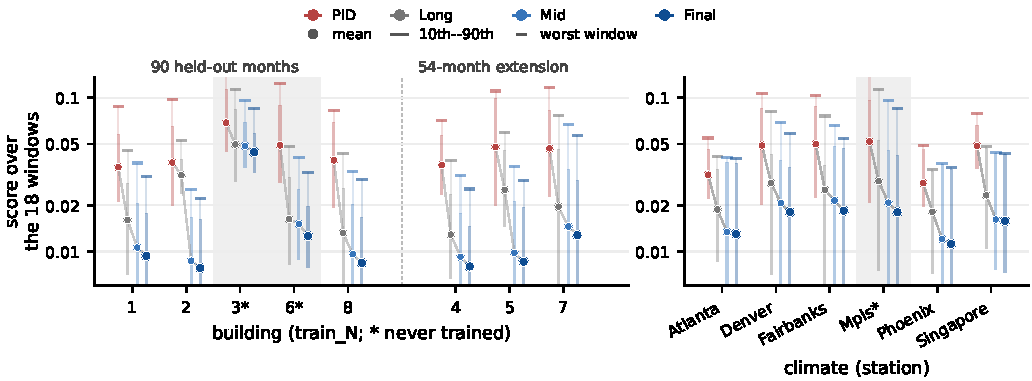
\includegraphics[width=\linewidth]{figures/fig_results_breakdown4_v2.pdf}
\caption{Every building and every climate, four policies. The dot is the mean over the 18 held-out windows of that building or station, the line the 10th to 90th percentile, and the tick the worst window; lower is better. The left block is the 90-month set, the right block the 54-month extension. A star marks a building or station never trained. The order of the four policies is the same inside every range.}
\label{fig:breakdown}
\end{figure}

Figure~\ref{fig:breakdown} shows the distribution behind each mean. Final's worst window is 0.0855 against 0.0960 for Mid, 0.1131 for Long and 0.1625 for PID. \texttt{train\_3} owns all five of its worst months and a fifth of the total (Appendix~F); its 47\% in-band share against 84--98\% elsewhere (Appendix~H) is the residual, not a policy-wide comfort failure. The split is computed on the $5\times18$ grid of month scores: 74\% building identity, 22\% weather window and 4\% interaction.

On the 54-month extension the buildings are three it trained on, and the windows are the same 18 unseen months. Final is 0.0098, below Mid (0.0112), Long (0.0192) and PID (0.0437) on all 54. The gain is comfort first: occupied zone-steps sit in band 84--98\% of the time on four buildings, \texttt{train\_3} is at 47\%, and the drop against Long is 76\% comfort, 9\% energy and 15\% carbon, while comfort is still 42\% of Final's score, energy 31\% and carbon 27\%. Electricity falls on every building, 73.3 to 45.2\,MWh, gas on three of five, 95.6 to 89.1, and CO$_2$ on four of five, 24.6 to 20.6\,t; gas rises in the two largest plants and CO$_2$ in one, so the total is not a fuel swap (Appendix~G).

\subsection{By time of day and by month}

Final is cheapest while the building is occupied: 0.021--0.041 per step between 06:00 and 19:00, against 0.024--0.045 for Mid, 0.038--0.051 for Long and 0.066--0.131 for PID. At 06:00, the hour the building fills, it is 0.041 against 0.045, 0.051 and 0.131. The weekday night is the only bin where Final is worse than PID, by 20\% (0.0045 against 0.0037); Mid and Long are worse there, 0.0064 and 0.0049.

Figure~\ref{fig:time} breaks the same recording three ways. By hour, the four separate in the occupied window and converge at night. By day-part, the weekday morning is the largest bill for every policy, and weekends are 29\% of the steps with 0.2\% of the electricity and 0.7\% of the gas. By month, the cold windows carry the bill and the warm ones are nearly free; Final is lowest in every month, from 0.033 in January to 0.009 in August, and \texttt{train\_3} drifts by $3.8\times10^{-4}$ per day, about 0.011 over the month (Appendix~H).

\begin{figure}[h]
\centering
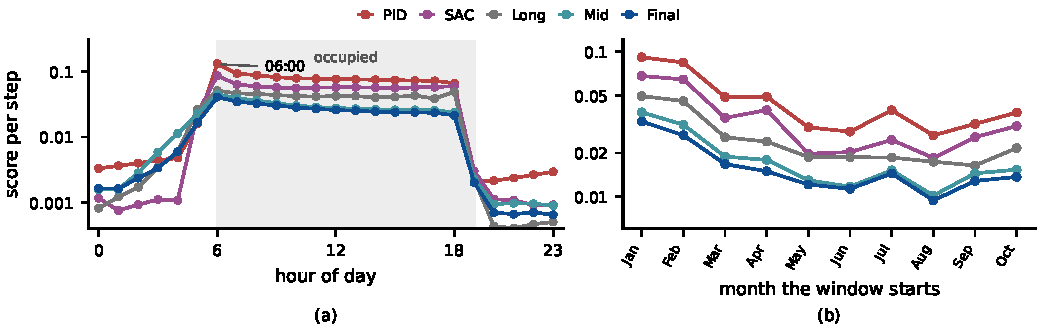
\includegraphics[width=0.9\linewidth]{figures/fig_results_time4.pdf}
\caption{The same recording by hour, by day-part and by month. (a) Score per step by hour of day, on a log scale; the shaded band is the occupied window, and 06:00 is the most expensive hour for every policy. (b) Weekday night, morning, afternoon and evening and the weekend, log scale. (c) The month each window starts, January to October. Lower is better throughout.}
\label{fig:time}
\end{figure}

It does not save by switching equipment off; it saves by choosing when the building is conditioned (Appendix~H).

\section{Conclusion}
\label{sec:conclusion}

A single 453K-parameter policy, trained once across six buildings and five climates, was evaluated across eight buildings and six climates. It achieves scores of 0.0165 on the 90 held-out months and 0.0098 on the 54-month extension, compared to 0.0461 and 0.0437 for the benchmark's default controller. More consequential than the mean score is its variance structure: 74\% of the score spread is attributable to building identity and only 22\% to weather, directly inverting the baseline's sensitivity. The policy decouples control performance from seasonal variation, leaving building-specific dynamics as the primary residual.

Three things bound that claim. It is one seed. Some noise remains in the reported score, and the recipe was not tested with ablations at this scale, one change at a time. And the baseline is the controller the benchmark ships, untuned: no tuned classical controller and no other reinforcement-learning algorithm was run against it.

Three tests follow. First, our reported experiments were conducted on the original, \textbf{unpatched} benchmark release; this comparison must be replicated on the corrected environment alongside official entrant submissions. Second, multi-seed evaluations are required to quantify performance variance. Third, the policy must be benchmarked against stronger reinforcement learning baselines.


\clearpage
\bibliographystyle{unsrtnat}
\nocite{*}
\bibliography{references}

\clearpage
\appendix

\section{Simulator, validation and throughput}
\label{app:sim}

\subsection{The port}
\label{app:port}

The policy is trained inside a CUDA port of the benchmark's simulator. The port replaces the finite-difference thermal network, the convection coupling, the sparse solve, the occupancy model and the reward, and it exposes the environment through PufferLib's vector interface, so a rollout step is one launch per subsystem and a whole update is capturable as a graph. The physics is not approximated: same cells, same boundary conditions, same solver.

The model is the benchmark's. Every control volume is a finite-difference thermal network with an internal mass node for the slab, floor and furniture, coupled by convection to the zone air, given the commands and the scenario's weather trace the state advances deterministically, and randomness enters only through per-zone occupancy, which evolves as Markov chains of Bernoulli arrivals and departures inside each zone's operating window.

\subsection{Validation}
\label{app:validation}

\begin{table}[h!]
\centering
\small
\begin{tabular}{@{}lll@{}}
\toprule
check & comparison & result \\
\midrule
reset observation & port vs reference, per scenario & 0 differing values \\
observation, every step & port vs reference, 30 scenarios, 8{,}640 steps & 0 differing values \\
reward, every step & port vs reference, same runs & 0 differing values \\
thermal solve & port vs CPU replay & differs by about $2\times10^{-14}$ \\
canonical slot map & slots used vs native action count & equal for all six buildings \\
action mask & active heads vs present slots & equal \\
episode length and terminals & port vs reference & equal \\
\bottomrule
\end{tabular}
\vspace{4pt}
\caption{The port against the reference Python implementation. The first three rows are exact comparisons, value by value; the fourth is the only place the two differ.}
\label{tab:app_validation}
\end{table}

Only the solve differs, and it differs because the summation order differs: a floating-point sum over a sparse factorisation is not associative. Everything the gateway hands the policy and everything the policy is paid is reproduced exactly, which is what makes it legitimate to score an episode on the GPU.

\subsection{Throughput}
\label{app:throughput}

\begin{table}[h!]
\centering
\small
\begin{tabular}{@{}llrr@{}}
\toprule
configuration & hardware & agents & steps/s \\
\midrule
30 scenarios, 32 agents each & NVIDIA L40S, 46\,GB & 960 & 12.0K \\
4 scenarios, 64 agents each & NVIDIA RTX 3090, 24\,GB & 256 & 6.2K \\
reference Python, 12 CPU cores & AMD Ryzen 5700F & 12 & 145 \\
\bottomrule
\end{tabular}
\vspace{4pt}
\caption{Measured environment steps per second, double-precision physics in every row. The reported run uses the 960-agent L40S row.}
\label{tab:app_throughput}
\end{table}

\subsection{Build and run}
\label{app:build}

Everything is built and executed inside the \texttt{pufferai/puffertank:5.0} image. The reported run used one frozen executable whose digest is recorded with its checkpoints, and its data archive is verified at start-up; a mismatch aborts rather than trains. Evaluation always uses the double-precision path. A single-precision solve exists as an opt-in speed experiment; it is not used for training here either, because its observation differs from the double-precision reference by about $10^{-4}$ and the reward a policy would be trained on would not be the reward this paper reports.

\section{The input contract}
\label{app:contract}

The policy never sees a building's own observation vector. It sees this one: 90 zone slots of 9 values, 9 air-handler slots of 16, one plant slot of 10 and one global slot of 19. Zone slot $s = 10k + j$ is the $j$-th zone served by air handler $k$, with handlers in numeric id order and zones in the order their temperature sensor first appears. Slots past a building's counts are zero, which is what makes the vector comparable across buildings; every slot except the global one starts with a presence flag, so a zero there means ``this equipment does not exist'' rather than ``this equipment reads zero''. No PID or rule-based controller is used anywhere in the policy: no action is a residual on one, no head is initialised to reproduce one, and no filter or override of its commands exists.

\begin{figure}[h!]
\centering
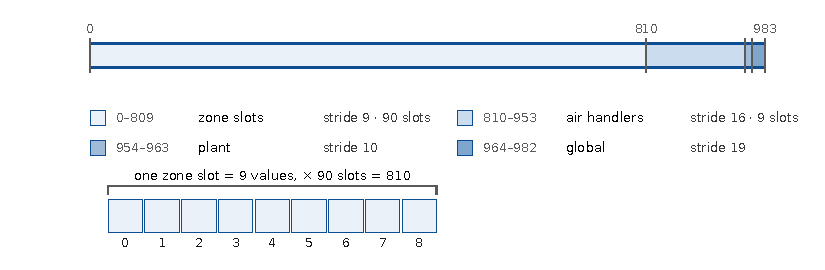
\includegraphics[width=0.95\linewidth]{figures/fig_appendix_slots.pdf}
\caption{The 983-value vector as an address map (top) and as one slot (bottom). Offsets run 0--809 for the 90 zone slots, 810--953 for the 9 air-handler slots, 954--963 for the plant and 964--982 for the global slot, and the legend gives each group's stride. The lower row expands a single zone slot; the numbers under it index the nine values of Table~\ref{tab:app_zone_values}, where 7 and 8 are the benchmark's controller commands and the rest are sensors and command echoes.}
\label{fig:appendix_slots}
\end{figure}

\subsection{Zone slots}
\label{app:zone}

\begin{table}[h!]
\centering
\small
\begin{tabular}{@{}rlcl@{}}
\toprule
\# & value & scaling & source \\
\midrule
0 & presence & $1/0$ & equipment map \\
1 & zone air temperature & $(T-295)/5$ & sensor \\
2 & heating setpoint shortfall & $(T-H_s)/2$ & sensor and setpoint \\
3 & cooling setpoint headroom & $(C_s-T)/2$ & sensor and setpoint \\
4 & heating setpoint & $(H_s-294)/3$ & setpoint \\
5 & damper position & $2D-1$ & command echo \\
6 & reheat valve & $2R-1$ & command echo \\
7 & the controller's damper command & $[-1,1]$ & \texttt{pid\_water} \\
8 & the controller's reheat command & $[-1,1]$ & \texttt{pid\_water} \\
\bottomrule
\end{tabular}
\vspace{4pt}
\caption{The nine values of one zone slot. $T$ is the zone temperature, $H_s$ and $C_s$ its heating and cooling setpoints, $D$ and $R$ its damper and reheat commands. Rows 7 and 8 are the benchmark's controller commands, which the policy does not read.}
\label{tab:app_zone_values}
\end{table}

\subsection{Air-handler, plant and global slots}
\label{app:ahu}

The gateway supplies twelve harmonics per family; the canonical layout keeps the first four sine and the first four cosine of each, sixteen values in all, which is the ``16 retained'' line of Table~\ref{tab:interface}.

One choice in this layout is measured rather than assumed: the comfort deficits are stored as magnitudes, not as signed values. The signed variant, which would let a zone that is too hot excite the cold shortfall that opens its reheat valve, costs 33\% of the ten-month panel and is worse at all six saves.

\begin{table}[h!]
\centering
\small
\begin{tabular}{@{}rlcl@{}}
\toprule
\# & value & scaling & source \\
\midrule
0 & presence & $1/0$ & equipment map \\
1 & outdoor air temperature & $(T_{oa}-283)/15$ & sensor \\
2 & supply-air static pressure & $P/1000$ & sensor \\
3 & supply-air flowrate & $F/10$ & sensor \\
4 & outdoor-air flowrate & $F/10$ & sensor \\
5 & supply-air temperature setpoint & $(T_s-295)/5$ & setpoint \\
6 & recirculation & $2R-1$ & command echo \\
7 & cooling request count & $C/10$ & equipment \\
8 & run command & $2u-1$ & command echo \\
9--12 & the controller's four air-handler commands & $[-1,1]$ & \texttt{pid\_water} \\
13 & mean zone temperature of the group & $(\bar T-295)/5$ & aggregate \\
14 & base-controller PID error & $/10$ & \texttt{pid\_water} \\
15 & base-controller effort & $[0,1]$ & \texttt{pid\_water} \\
\bottomrule
\end{tabular}
\vspace{4pt}
\caption{The sixteen values of one air-handler slot. $T_{oa}$ outdoor air temperature, $P$ static pressure, $F$ flowrate, $T_s$ supply-air temperature setpoint, $R$ recirculation, $C$ cooling request count, $u$ run command. Rows 9--12 are the controller's four air-handler commands, which the policy does not read.}
\label{tab:app_ahu}
\end{table}

\begin{table}[H]
\centering
\small
\begin{tabular}{@{}rlcl@{}}
\toprule
\# & value & scaling & source \\
\midrule
\multicolumn{4}{@{}l}{\emph{plant slot (10)}} \\
0 & presence & $1/0$ & equipment map \\
1 & supply-water temperature & $(T-330)/20$ & sensor \\
2 & supply-water temperature setpoint & $(T-330)/20$ & setpoint \\
3 & differential pressure & $P/10$ & sensor \\
4 & differential pressure setpoint & $P/10$ & setpoint \\
5 & run status & $2r-1$ & status \\
6 & heating request count & $/10$ & equipment \\
7--9 & the controller's three plant commands & $[-1,1]$ & \texttt{pid\_water} \\
\multicolumn{4}{@{}l}{\emph{global slot (19)}} \\
0--3 & hour harmonics, sine & as supplied & calendar \\
4--7 & hour harmonics, cosine & as supplied & calendar \\
8--11 & day-of-week harmonics, sine & as supplied & calendar \\
12--15 & day-of-week harmonics, cosine & as supplied & calendar \\
16 & comfort mode now & $0/1$ & schedule \\
17 & comfort mode in 60 minutes & $0/1$ & schedule \\
18 & building occupancy & occupants & sensor \\
\bottomrule
\end{tabular}
\vspace{4pt}
\caption{Plant and global slots. The plant slot is the hot-water loop; the global slot carries the only calendar information the policy receives and the only building-wide occupancy information. Rows 7--9 are the controller's three plant commands, which the policy does not read.}
\label{tab:app_plant}
\end{table}

\subsection{Field identifiers, collisions and missing values}
\label{app:fields}

A field identifier is the device id joined to the measurement name. When that string already belongs to another pair the gateway appends \texttt{\_1}, so an identifier is unique but not parseable by pattern; the canonical map is built from the identifier list in device order, never by matching a regular expression. A missing measurement is filled from the previous observation rather than zeroed, because a zero in a temperature field is a plausible temperature and would silently corrupt the features. Neither rule is learned; both are applied identically at training and at evaluation.

\subsection{The reward's schedules}
\label{app:reward}

The comfort term is the only unbounded one. A zone that sits far outside its band costs more than the entire energy and carbon bill of a good month, which is why the tail of the score, not its mean, is the quantity a practitioner should watch.

Every one of the 983 values is named and scaled, and the schedule the reward is computed from is the benchmark's own rather than one we chose.

\begin{table}[h!]
\centering
\small
\begin{tabular}{@{}lll@{}}
\toprule
quantity & form & range over the 90 months \\
\midrule
electricity price & hourly, weekday and weekend schedules & 16--20\,¢/kWh \\
gas price & one constant per month & monthly schedule \\
grid carbon intensity & hourly schedule & 87.8--104.7\,g/kWh \\
gas emission factor & constant per joule & 0.1813\,kg/kWh \\
comfort term & \$300 per occupant-hour, 5\,K linear then quadratic & unbounded below \\
comfort band & occupied and unoccupied setpoints & per building \\
\bottomrule
\end{tabular}
\vspace{4pt}
\caption{The quantities the reward is computed from. All are the benchmark's, unchanged; the ranges are what the 90 held-out months contain.}
\label{tab:app_reward}
\end{table}

\section{Delay features and the memory}
\label{app:delay}

\begin{figure}[h!]
\centering
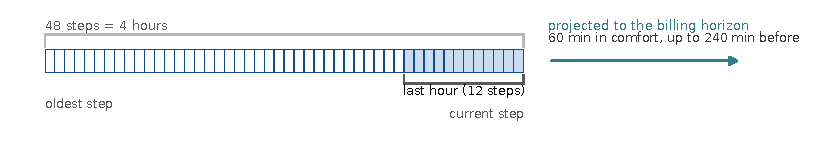
\includegraphics[width=0.8\linewidth]{figures/fig_appendix_memory.pdf}
\caption{The per-zone memory. Each zone keeps its last 48 temperature and deficit samples, four hours at five minutes per step, and projects its own trajectory forward to the moment the delayed reward is billed: sixty minutes while comfort is active, up to four hours while the building waits for occupancy.}
\label{fig:appendix_memory}
\end{figure}

A setpoint change is paid for hours later, and the thermal mass that delays the bill is not in the observation. Each zone therefore carries a short history of itself and a projection of where it is heading, both computed from the gateway vector alone.

\subsection{The ring}
\label{app:ring}

Each zone slot carries a ring of 48 samples of its own temperature and of its distance outside the comfort band. The ring is empty at the first step and fills as the episode runs, so the history-derived features become informative once one hour of history exists; the four entries taken from the observation itself are valid from step one.

\subsection{The eleven features}
\label{app:features}

\begin{table}[h!]
\centering
\footnotesize
\setlength{\tabcolsep}{4pt}
\begin{tabular}{@{}rlp{0.5\linewidth}c@{}}
\toprule
\# & feature & definition & clip \\
\midrule
0 & minutes to comfort start & $t_{\text{start}}/180$ & -- \\
1 & minutes to comfort end & $t_{\text{end}}/180$ & -- \\
2 & next-day flag & comfort starts more than a day away & 0/1 \\
3 & outdoor temperature change & $\Delta T_{oa}/2$ over one step & -- \\
4 & current deficit & band distance $/5$ & -- \\
5 & mean deficit over the last hour & mean of 12 samples $/5$ & -- \\
6 & mean deficit over the ring & mean of up to 48 samples $/5$ & -- \\
7 & temperature slope & K per hour, from the ring & -- \\
8 & mean temperature over the ring & $(\bar T-295)/5$ & -- \\
9 & deficit projected to billing & band distance of $T+\text{slope}\cdot h$ & $\le 10$ \\
10 & fan path & damper $\times(H_s-T)/5$, reheat $<0.3$, supply $\le T$ & $\le 10$ \\
\bottomrule
\end{tabular}
\vspace{4pt}
\caption{The engineered features appended to each zone slot, after the nine of Table~\ref{tab:app_zone_values}, the eight air-handler values it inherits and its comfort deficits. The last two are the ones that close the delay.}
\label{tab:app_features}
\end{table}

Feature 9 is the delay closed in the state: $h$ is 60 minutes while comfort is active and $\min(t_{\text{start}},240)$ while it is not, so the feature asks ``how far out of band will this zone be when the reward is charged?'', not ``how far out is it now''. Feature 10 is the second half of the same argument: a damper held open on a zone that is already below its heating setpoint, with the reheat valve closed and supply air no warmer than the room, means the fan is doing the heating and the electricity for it is billed later. Both are clipped at ten so a single frozen zone cannot dominate the input.

What these features are worth is measured, and the honest answer is split. The critic was given its own eight-number summary of the same quantities, and removing it improves the ten-month panel by 9\,\% and is better at all six saves: presented to the critic, the delay numbers add nothing, which is consistent with the earlier finding that the critic ranks time well and rooms poorly. The actor keeps the projection and the fan path, because those are the features the action is chosen from, and the loop is closed through the reward. What we have not done is isolate the actor's block with a single-flag arm at the final recipe, and we say so rather than implying a measured gain for it. The ring and the projection are therefore described here as a design that encodes the delay, not as a component with an attributable score contribution.

\subsection{What resets at an episode boundary}
\label{app:reset}

The ring, its sample count and the outdoor-temperature memory are cleared at every episode boundary. The comfort schedule and occupancy are not, because they come from the gateway vector. Nothing is carried across scenarios, so the policy cannot recognise a building from its history.

Every number in the input is named, scaled and reproducible from the gateway vector, and the two quantities that close the delayed reward, the projected deficit and the fan path, are computed from that vector alone, reset with the episode, and clipped so that one zone cannot dominate.

\section{The action distribution and the optimizer}
\label{app:action}

Up to 219 heads draw from one trunk, so two properties decide whether the arrangement trains at all: whether a head can sit at the end of its range without losing the gradient that would bring it back, and whether one head can be corrected without moving the others. Both are properties of the distribution and of the update rule rather than of the network's width, and both were measured at the final recipe, one change per arm.

\begin{figure}[h!]
\centering
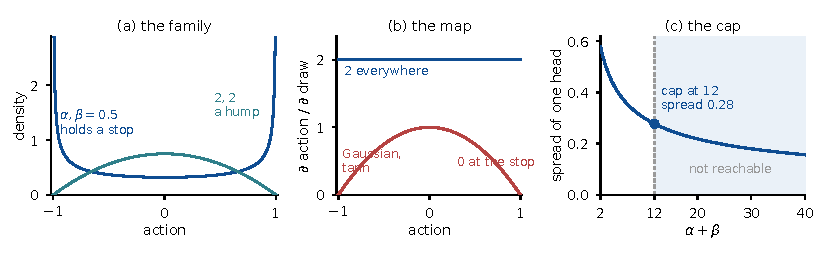
\includegraphics[width=0.95\linewidth]{figures/fig_appendix_beta.pdf}
\caption{The shape of one control head. (a) A Beta with both parameters below one puts its mass at the two stops, which is how a damper is held shut or a valve held open; with both above one it is a hump, which is how a command tracks a setpoint. (b) The tanh map that a squashed Gaussian needs has derivative $1-a^2$, which is 0.10 at nine tenths of the range and 0 at the stop; the Beta's affine map has the same sensitivity everywhere. (c) The spread of a head falls as $\alpha+\beta$ rises, so without a cap the policy can make a head arbitrarily certain; the cap at 12 holds the spread at 0.28 action units.}
\label{fig:appendix_beta}
\end{figure}

\subsection{A support that is the actuator range}
\label{app:support}

A continuous command is a physical interval: a damper from shut to open, a valve from closed to full flow. The obvious parameterisation, a Gaussian squashed by a tanh, fails at the two ends. To command a damper fully shut, the pre-squash mean has to move far into the tail, and the derivative of the map, $1-a^2$, falls to zero as it does (Figure~\ref{fig:appendix_beta}b), so the gradient that would move the damper off the stop vanishes exactly where holding it is the decision. The action's log-density also carries the term $-\log(1-a^2)$, which diverges at the stops, so a positive-advantage sample at the boundary contributes an unbounded quantity that has nothing to do with the building.

A Beta on $(0,1)$ has neither problem. Its support is the range, the map $a = 2x-1$ is affine with sensitivity 2 everywhere, and no sample is clipped, so the command that is scored is the command that was drawn. The two shape parameters give the head a shape as well as a centre: with $\alpha,\beta<1$ the density is U-shaped and puts mass at both stops, which is how a damper is held fully shut or fully open; with $\alpha,\beta>1$ it is a hump, which is how a command tracks a setpoint (Figure~\ref{fig:appendix_beta}a). The 0.5 floor on each parameter is what keeps the U-shape reachable; the cap in the next subsection bounds the other direction.

We moved to this parameterisation for a behavioural reason, not for a score. Our earlier implementation used the squashed Gaussian, settled into a cold operating point and did not leave it; the Beta variant, whose support covers the whole range and whose width can reopen, did. The state belongs to a month, not to the batch: the runs that separated the two were on one cold-demand month (Fairbanks), and in the reported run it appears on a single month, \texttt{train\_1/fairbanks\_1}, which sat at a month score of 5.3 for about 60M steps until the anneal moved it. In that state the dampers sit nearly shut, the reheat valves nearly fully open and recirculation at its cap. That observation precedes every arm in this appendix, so it is the motivation and not a measurement.

\subsection{A cap on certainty}
\label{app:cap}

A Beta with a large $\alpha+\beta$ is a needle, and a needle is a policy that has stopped exploring the head. The cap rescales both parameters by $12/(\alpha+\beta)$ when their sum would exceed 12, which lowers the concentration while leaving the mean $\alpha/(\alpha+\beta)$ unchanged. At mean one half this holds the spread of a head at 0.28 action units (Figure~\ref{fig:appendix_beta}c); without the cap the spread keeps falling towards a point mass.

The cap is worth 64\% of the panel. Removing it moves the final score from 0.033 to 0.054, worse at all six saves, and the early panel (2.18 at 10M against 0.273) is the hot-month lock returning: a run that has committed to one operating point so hard that it cannot sample its way out. The cap is not a reward regulariser and does not touch the score; it bounds how certain a head may become, which is a property of the search.

\subsection{One ratio per head}
\label{app:ratio}

The heads are not independent draws, but they are not one draw either. With a single joint ratio the update compares the product of the active densities, and two heads that move in opposite directions cancel in that product: a head at 1.30 and a head at 0.80 multiply to 1.04, inside the trust region, so a joint clip fires on neither and the zone head that has to correct itself is not allowed to.

Each head therefore keeps its own ratio, clipped on its own, so the surrogate is a sum over heads rather than a product over heads:
\[
\tilde r_h(\theta) = \mathrm{clip}\!\left(\frac{\pi_\theta(x_h\mid s)}{\pi_{\theta_{\text{old}}}(x_h\mid s)},\ 0.8,\ 1.2\right).
\]

Removing this is the second largest cost we measured: 0.152 against 0.033, and the shape of the curve is the argument. The arm without it is ahead at 20M (0.096 against 0.126) and then flat at 0.15 for the rest of the run while the unmodified recipe falls to 0.033, which is a policy that can raise the joint likelihood but cannot repair an individual zone. The mechanism was predicted before the arm ran, from the fraction of zone-head visits whose per-head ratio a sign-aware clip would catch on a Fairbanks month: 10.11\%.

None of this changes the reward, the executed action or the physics. It changes which parameter steps the estimator takes, and it is the only place where the heads are treated as separate decisions.

\subsection{An optimizer that adapts per weight}
\label{app:adam}

The earlier recipe ran Muon on the trunk and Adam only on the readout rows, on the argument that an orthogonalised update needs a per-weight correction on the small matrices it feeds. Both halves of that arrangement are measured. Remove the readout Adam while the trunk stays on Muon and the panel moves from 0.033 to 0.049, 48\% worse and worse at every save. Replace Muon with Adam everywhere and drop the split, and the panel moves to 0.029, better at all six saves and 41\% better than the arm that only dropped the split.

In this recipe the split behaves as a compensation rather than a component. Once the trunk's update adapts per weight, the correction it was there to provide has nothing left to correct, and keeping it is worse than dropping it. Our working explanation for why the compensation was needed is that the value tangent dominates the shared trunk by a measured factor of 20 to 400, so an update that equalises directions oversteps on the directions the value depends on, while a per-weight step size absorbs the difference. We state that as an explanation; what is measured is that Adam everywhere is better at the same wall clock, 6{,}018 against 6{,}069 steps per second.

\section{The training recipe and checkpoint selection}
\label{app:recipe}

Every arm in this section is trained from a fresh random initialisation, seed 75, for 50{,}135{,}040 steps, with the learning rate annealed linearly to zero over that same budget. Fourteen of them change one setting from the unmodified recipe and one changes several at once. The arms use the four-scenario batch (256 agents), because fifteen arms at the thirty-scenario scale would cost more than the reported run itself; the recipe was then trained at the thirty-scenario scale (960 agents) for the policy this paper reports. The read is the training panel, the mean episode score over the batch's scenarios on whole 8{,}640-step months, evaluated while the policy is still changing. It is a learning-curve statistic; it is not a frozen score, and it is not the held-out set.

\subsection{The batch and the schedule}
\label{app:batch}

Each update collects 288 steps from each of 960 environments, 276{,}480 transitions, and makes four passes of 120 minibatches of 2{,}304 samples, so one rollout is 480 gradient steps and the reported run is 723 rollouts. The learning rate starts at $10^{-4}$, is annealed linearly to zero over the full budget, and the reported checkpoint is taken at the end of that anneal, where the step size rather than the noise decides the final weights. Entropy carries a coefficient of 0.001 and was swept over 0, 0.005, 0.01 and 0.05 without a dose response, so it is left at its smallest effective value rather than tuned.

\subsection{Staggered episode starts}
\label{app:stagger}

The largest effect we measured is not a network or an optimizer choice but how the batch samples the calendar. With staggered starts every environment begins its month at its own phase, so a rollout contains many points of the seasonal and weekly cycle at once; with a common start all 960 environments sit at Sunday 06:00 and every update sees a single calendar state.

The measured cost of the common start is decisive: 2.213 against 0.033, worse at every save and never recovering (Figure~\ref{fig:appendix_ablation}). The mechanism is in the estimator, not in the environment. If every trajectory in a rollout is at the same point of the year, the advantage cannot separate ``this policy is worse in winter'' from ``this policy is worse'', and the update is left fitting the season rather than the behaviour. Staggering also produces episodes of different lengths in the first rollout, which is the only source of length diversity in the batch.

\subsection{What each change is worth}
\label{app:ablation}

\begin{figure}[h!]
\centering
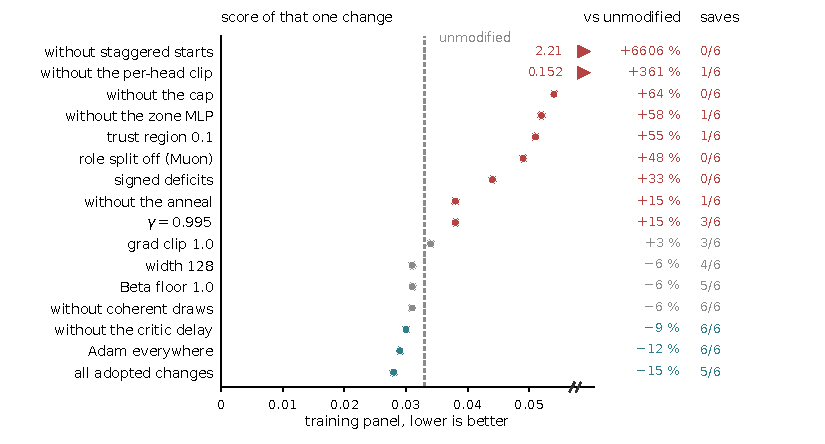
\includegraphics[width=0.72\linewidth]{figures/fig_appendix_ablation.pdf}
\caption{Fifteen single changes to the unmodified recipe and one arm that makes all the adopted changes at once, each trained for 50.1M steps from a fresh initialisation. The dashed line is the unmodified recipe at 0.033; a dot is the score with that one change and everything else left alone. Two changes score past the axis and are drawn as arrows with their values. A positive percentage means worse than the unmodified recipe and a negative one better.}
\label{fig:appendix_ablation}
\end{figure}

\begin{figure}[h!]
\centering
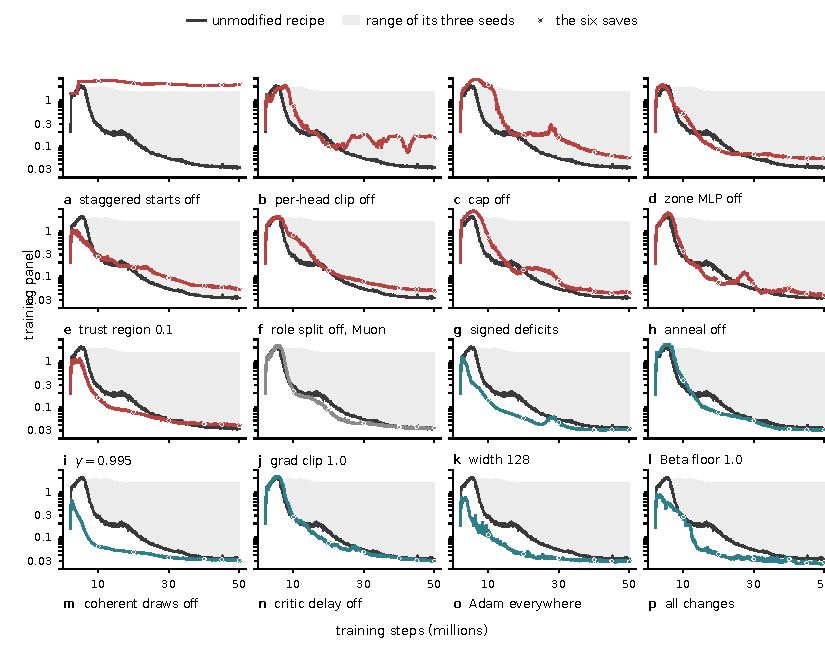
\includegraphics[width=0.98\linewidth]{figures/fig_ablation_A.pdf}
\caption{The curves behind Figure~\ref{fig:appendix_ablation}: each panel repeats one change (coloured) against the unmodified recipe (black) and the range of its three seeds (grey); dots mark the six matched saves and the ordinate is logarithmic. Lower is better. (a) staggered starts off: 2.21, no recovery. (b) per-head clip off: 0.152, ahead at 20M, flat from 30M. (c) cap off: 0.054, 2.18 at 10M. (d) zone MLP off: 0.052, 0.49 at 10M. (e) trust region 0.1: 0.051. (f) role split off under Muon: 0.049. (g) signed deficits: 0.044. (h) anneal off: 0.038, ahead at 20M, behind from 30M. (i) $\gamma=0.995$: 0.038. (j) grad clip 1.0: 0.034. (k) width 128: 0.031. (l) Beta floor 1.0: 0.031. (m) coherent draws off: 0.031. (n) critic delay off: 0.030. (o) Adam everywhere: 0.029. (p) all changes: 0.028.}
\label{fig:appendix_curve}
\end{figure}

Figure~\ref{fig:appendix_ablation} ranks the changes by their final value and Figure~\ref{fig:appendix_curve} shows the curves behind that ranking. Three of the changes matter more for their shape than for their endpoint. The per-head clip is ahead at 20M and then flat at 0.15 while the unmodified recipe falls to 0.033, so removing it costs the ability to repair a single zone. The cap goes the other way, a spike to 2.18 at 10M and a recovery that stops at 0.054: committing to one operating point early is expensive. $\gamma=0.995$ learns faster for the first 30M steps and converges worse after 40M, so the shorter horizon is kept; a trust region of 0.1 leads early in the same way and ends at 0.051. The coherence change counts once: zeroing either coherence time gives the same $-6\%$ and the same curve, so the two flags are one mechanism (correlated action sampling, \citealp{hollenstein2023colored}; \citealp{korenkevych2019autoregressive}). The last panel is the recipe the reported policy is trained with, Adam in place of Muon with the role split dropped, coherent draws off, the critic's delay summary removed and the Beta floor at 0.5; it reaches 0.042 at 20M where the unmodified recipe is at 0.126, ends at 0.0280 against 0.0330, and its last five readings stay between 0.026 and 0.028.

\subsection{Checkpoint selection}
\label{app:selection}

The reported policy is one of six saves. The rule was fixed before the held-out months were scored: take the save with the lowest training panel, and reject a save that lowers the mean only by blowing out the worst zone. The panel is the only signal available while training; the 90 months play no part in the choice.

The panel is a read of a policy that is still changing, which is why the choice matters. It stays between 0.07 and 0.26 for the first 120M steps and falls to 0.011 only after 145M, as the step size decays; a save at 120M reads 0.122, eleven times its value at the end. The panel selects the weights, and the deterministic month reports them.

The panel falls from 0.244 to 0.011 and the typical worst zone falls with it, from 3.30 to 1.81\,K. The worst single episode does not: it moves between 9.6 and 12.8\,K across the six saves, which is the noise of one window rather than a trend. The last two saves are therefore indistinguishable, with the same panel to three digits and a tail inside that noise (11.9 against 10.1\,K on the worst episode, 1.81 against 1.96\,K typical, 0.260 against 0.236 out of band). We report 199{,}065{,}600 because it is the last save with a complete diagnostic row; the final epoch was logged for the panel only.

\begin{figure}[h!]
\centering
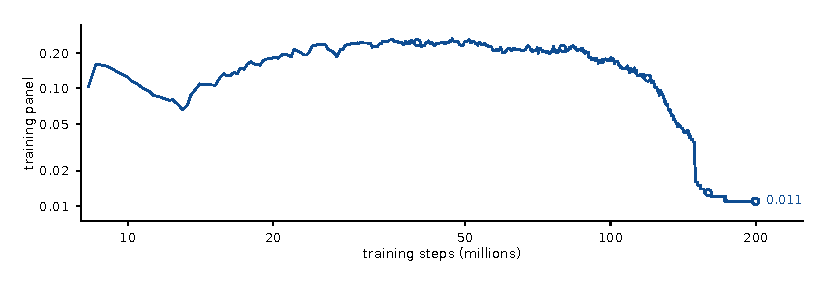
\includegraphics[width=0.90\linewidth]{figures/fig_appendix_curve.pdf}
\caption{The training panel of the reported run, one point per rollout, with the six saves marked. The ordinate is logarithmic, so the last decade gets the same room as the first: the panel stays near 0.2 for 120M steps, then falls to 0.011 after 145M as the learning rate decays. It is read over 30 scenarios and is not comparable with the four-scenario panels of Figures~\ref{fig:appendix_ablation} and~\ref{fig:appendix_curve}; the held-out score of the final checkpoint, 0.0165, is a third measurement on different months.}
\label{fig:appendix_panel}
\end{figure}

\begin{table}[h!]
\centering
\small
\begin{tabular}{@{}lrrrr@{}}
\toprule
save (M steps) & training panel & worst episode (K) & worst zone, typical (K) & out of band \\
\midrule
39.8 & 0.2435 & 12.41 & 3.30 & 0.334 \\
79.6 & 0.2177 & 12.77 & 3.28 & 0.309 \\
119.4 & 0.1224 & 11.73 & 2.99 & 0.315 \\
159.3 & 0.0128 & 9.65 & 1.98 & 0.203 \\
199.1 & 0.0109 & 10.07 & 1.96 & 0.236 \\
199.9 & 0.0109 & 11.9 & 1.81 & 0.260 \\
\bottomrule
\end{tabular}
\vspace{4pt}
\caption{The six saves of the reported run. ``Worst episode'' is the mean over episodes of the largest zone deviation reached in that episode; ``worst zone, typical'' is the mean over the last logging window of the per-step maximum; ``out of band'' is the fraction of zone-steps outside the comfort band. The last row's diagnostics are the last logged window, one epoch before that save.}
\label{tab:app_saves}
\end{table}

Two limits: the choice uses the training panel, not the held-out months, so the 90-month score is not a selection criterion; and there is one seed, so a difference between arms is not a distribution.

\section{Evaluation, the metric and the baseline}
\label{app:eval}

A month is reduced to one number, and the leaderboard to one number over months. For scenario $i$ with $T=8{,}640$ steps,
\[
S_i=\frac{1}{T}\left|\sum_{t=1}^{T}r_{i,t}\right|,\qquad \text{score}=\frac{1}{N}\sum_{i=1}^{N}S_i,
\]
where $r_{i,t}$ is the 3C reward of Section~3.1. Every term of $r$ is non-positive, so the absolute value only changes the sign: the score is the mean loss of one month, zero is the ideal, and the leaderboard is the mean of those losses over the graded months.

\subsection{Why the absolute value of a mean}
\label{app:abs}

The month is averaged inside the absolute value, first over time and then over scenarios, so every month is one vote and a building with 85 zones does not weigh four times one with 30. Averaging the absolute value at every step instead would charge the policy for the swing inside the month as well as for its level, and the competition charges the level. The result is not normalised per building either, so a building the policy controls badly arrives at full weight.

That makes the mean a weak summary when a few months are much worse than the rest, and those months are where this policy's remaining error sits (Figure~\ref{fig:appendix_scores}). Over the 90 months the mean is 0.0165 and the median is 0.0094; the five worst months are all the same building, the largest in the set, and they carry a fifth of the total. A report that quoted the median, or that averaged buildings before months, would hide that. We therefore report the mean, the per-building and per-climate breakdown of Figure~\ref{fig:breakdown}, and the tail beside it.

\begin{figure}[h!]
\centering
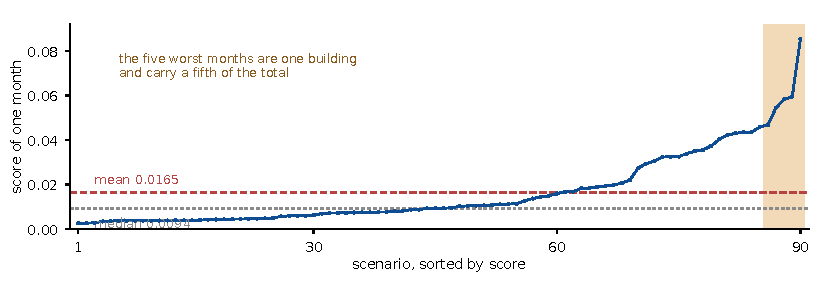
\includegraphics[width=\linewidth]{figures/fig_appendix_scores.pdf}
\caption{The ninety scored months, sorted. The metric is the mean of these values (dashed red), not their median (dotted grey). The shaded band is the five worst months: one building, a fifth of the total.}
\label{fig:appendix_scores}
\end{figure}

\subsection{The deterministic evaluator}
\label{app:det}

Each scenario is one episode of 8{,}640 steps in double precision, starting at the scenario's own timestamp, with the action set to the mean of each Beta head rather than a sample: no exploration noise, no early termination and no second seed. A scenario therefore has one trajectory, and every spread in this paper is across scenarios, not across runs.

The evaluator writes the observation, the executed action, the reward, its three terms and the per-step diagnostics, and every table in the results section is computed from those recordings rather than from a second episode. The submitted policy is a CPU re-implementation of the same weights; on two held-out months it reproduces the GPU score to within $3\times10^{-4}$, which is what makes a local month and a graded month the same measurement.

\subsection{What the baseline is}
\label{app:baseline}

\texttt{pid\_water} is the benchmark's water-based PID controller: a proportional-integral loop on each zone's temperature error, driving the water valve and the damper, with a supply-water reset. It reads the same observation and it has no term for price or carbon.

\begin{table}[h!]
\centering
\small
\begin{tabular}{@{}lrr@{}}
\toprule
controller & scenarios & score \\
\midrule
\multicolumn{3}{@{}l}{\emph{the 30 shipped scenarios, each controller as supplied}} \\
\texttt{bang\_bang} & 30 & 0.2252 \\
\texttt{pid} & 30 & 0.0674 \\
\texttt{fixed\_setpoint} & 30 & 0.0659 \\
\texttt{pid\_water} & 30 & 0.0541 \\
\multicolumn{3}{@{}l}{\emph{the 90 held-out months this paper scores}} \\
\texttt{pid\_water} & 90 & 0.0461 \\
this policy & 90 & 0.0165 \\
\bottomrule
\end{tabular}
\vspace{4pt}
\caption{The shipped controllers on the benchmark's own scenarios, and the two numbers this paper compares. The blocks are different scenario sets: a score may be compared inside a block, never across it.}
\label{tab:app_baseline}
\end{table}

It is the controller the benchmark ships, not one we tuned: every gain is the default. We say so because a tuned PID would be a stronger opponent, and because the claim is only that the learned policy is better than the controller the benchmark supplies. The gap is not uniform. On one window (\texttt{singapore\_4}) the shipped \texttt{fixed\_setpoint} controller scores 0.024 against \texttt{pid\_water}'s 0.108, so the PID is not the best classical controller everywhere, and it is the one we happened to beat by the largest margin.

\subsection{The public leaderboard}
\label{app:public}

All four policies have a public score. The public split is the third of the hidden evaluation the competition publishes, 48 scenarios; the other two thirds are private and we do not see them. The scores are the public column of Table~\ref{tab:score}: Mid 0.0175, Long 0.0182, Final 0.0294 and \texttt{PID} 0.0640, so every learned save is below the controller. Among the three, the split ranks Mid first and Final last, the reverse of the 90 and 54 months.

The reversal is a property of the split rather than evidence that the final save is worse. A mean over 48 months is more sensitive to a single bad month than a mean over 90, and the only local quantity that orders the two saves the way the public split does is the worst-episode excursion, 9.65\,K for Mid against 10.07\,K for Final (Table~\ref{tab:app_saves}); on the 90 months Final is the better of the two. The public score is therefore reported beside the local sets and never instead of them, and the policy this paper reports is the last save of the anneal (Appendix~\ref{app:selection}), not the public favourite.

\section{Buildings and climates}
\label{app:buildings}

One set of 453K weights serves eight buildings and six weather stations. Six buildings crossed with five stations, one month per pair, is the training set; the evaluation crosses five buildings with eighteen windows, and two of those buildings and one of those stations never appear in training. Buildings differ in size, plant count, envelope and occupancy; they do not differ in the interface they are written into (Appendix~\ref{app:contract}).

\begin{table}[h!]
\centering
\small
\begin{tabular}{@{}lrrrrrr@{}}
\toprule
building & zones & air handlers & zones per handler & floors & floor area (10$^3$ ft$^2$) & commands \\
\midrule
\texttt{train\_1} & 39 & 4 & 9.8 & 3 & 210 & 97 \\
\texttt{train\_2} & 85 & 9 & 9.4 & 2 & 253 & 209 \\
\texttt{train\_4} & 54 & 6 & 9.0 & 3 & 272 & 135 \\
\texttt{train\_5} & 79 & 8 & 9.9 & 4 & 271 & 193 \\
\texttt{train\_7} & 36 & 4 & 9.0 & 2 & 142 & 91 \\
\texttt{train\_8} & 30 & 3 & 10.0 & 2 & 126 & 75 \\
\midrule
\texttt{train\_3} & 70 & 7 & 10.0 & 3 & 837 & 171 \\
\texttt{train\_6} & 43 & 6 & 7.2 & 2 & 390 & 113 \\
\bottomrule
\end{tabular}
\vspace{4pt}
\caption{The eight buildings. ``Commands'' is the number of continuous actuators the gateway accepts: two per zone, four per air handler and three for the plant. The last two rows were generated with their own geometry and materials for the evaluation and were never trained on.}
\label{tab:app_buildings}
\end{table}

\subsection{The buildings}
\label{app:building_text}

The six trained buildings span 30 to 85 zones, 3 to 9 air handlers, 2 to 4 floors and 126 to 272 thousand square feet of floor area, and the number of continuous commands spans 75 to 209. Occupancy differs by design: 8 to 31 people on average across the five evaluated buildings, and a fixed 36\% of the month carries an occupant in every one of them, so the comfort term is billed on the same share of time whatever the building.

The two generated buildings are not at the ends of the range. They were built with their own materials and geometry and sit in the middle and upper middle of the plant-size range, so the unseen pair is not ``small versus new''.

\subsection{The climates}
\label{app:climates}

Five stations are trained, from Fairbanks and Denver through Atlanta and Phoenix to Singapore, and Minneapolis enters only at evaluation. Demand is measured in degree-days, the sum over the month of how far the outdoor temperature sits below 18\,$^\circ$C or above 21\,$^\circ$C. Across the 48 months the heating demand runs from 0 to 1182 and the cooling demand from 0 to 475, and the mixed months need both.

Figure~\ref{fig:appendix_climate} is the precise statement of what ``unseen weather'' means here. Nine of the ten scored windows at a trained station fall inside that station's trained range; the tenth, Denver's January window, carries 46\% more heating demand (567 degree-days against a trained maximum of 389) than any Denver month the policy saw. Minneapolis has no trained range: eight scored months, no trained month. The two kinds of novelty, a colder month at a known station and a whole new station, are not the same test.

\begin{figure}[h!]
\centering
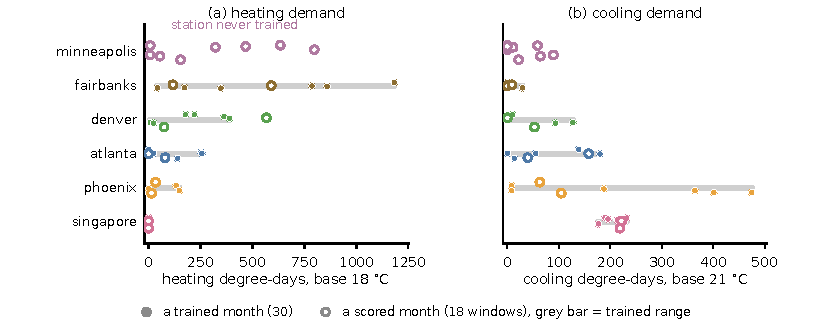
\includegraphics[width=0.95\linewidth]{figures/fig_appendix_climate.pdf}
\caption{The 48 months. Each row is a station; the grey bar is the range of the months trained on there, filled circles are trained months and open circles are scored months.}
\label{fig:appendix_climate}
\end{figure}

\subsection{What is held out}
\label{app:holdout}

Two of the eight buildings, one of the six stations and all 18 windows are held out: every scored window is a calendar month that never appears in the 30 training scenarios. The check is by name as well as by construction: 0 of the 90 scenario names occurs in any training batch (Figure~\ref{fig:appendix_coverage}).

Two limits belong beside that claim. The training set is a design rather than a sample: one month per building-station pair, chosen to cover the year, so the policy never sees two consecutive months at one station. And the evaluation set is a design too, two windows per trained station plus eight for Minneapolis, so its station balance is not the competition's. Both are the right choice for a controlled comparison and neither is a random draw from the year.

\begin{figure}[h!]
\centering
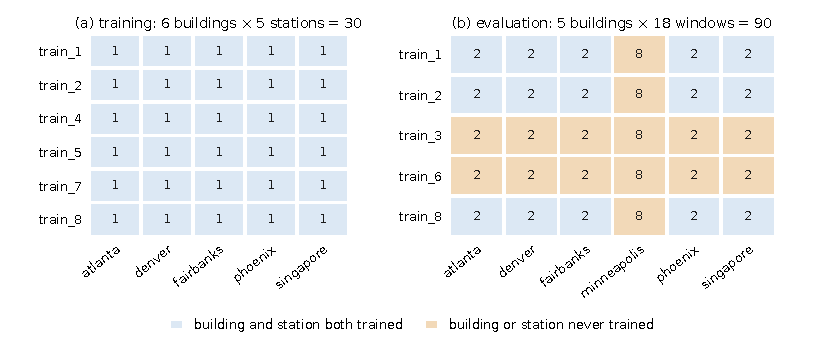
\includegraphics[width=\linewidth]{figures/fig_appendix_coverage.pdf}
\caption{Coverage of the two sets. (a) the 30 training scenarios, one month for each building-station pair. (b) the 90 scored months: five buildings, two windows per trained station and eight for Minneapolis. Orange marks a cell in which the building or the station was absent from training.}
\label{fig:appendix_coverage}
\end{figure}

\subsection{The 54-month extension}
\label{app:extension}

The three shipped buildings missing from the 90-month set, \texttt{train\_4}, \texttt{train\_5} and \texttt{train\_7}, are scored on the same 18 windows, 54 months in all. All four policies are scored on them. The extension is never pooled with the 90; the two sets sit side by side in Table~\ref{tab:score}. Per building, the means are 0.0080, 0.0086 and 0.0128 for Final; 0.0092, 0.0098 and 0.0145 for Mid; 0.0129, 0.0252 and 0.0196 for Long; and 0.0365, 0.0478 and 0.0469 for \texttt{PID}. The ordering is the same as on the 90.

\subsection{What the score is made of}
\label{app:fuel}

The term drops against Long and the composition of the remaining score are computed row by row from Table~\ref{tab:score}; comfort is the largest term in every policy and the one that falls most. Table~\ref{tab:app_fuel} gives the per-building fuel and CO$_2$ behind the totals in the text.

\begin{table}[h!]
\centering
\small
\begin{tabular}{@{}lrrrrrr@{}}
\toprule
 & \multicolumn{2}{c}{electricity (MWh)} & \multicolumn{2}{c}{gas (MWh)} & \multicolumn{2}{c}{CO$_2$ (kg)} \\
\cmidrule(lr){2-3}\cmidrule(lr){4-5}\cmidrule(lr){6-7}
building & Final & \texttt{PID} & Final & \texttt{PID} & Final & \texttt{PID} \\
\midrule
\texttt{train\_8} & 2.8 & 6.2 & 9.8 & 17.6 & 2{,}064 & 3{,}802 \\
\texttt{train\_1} & 4.7 & 7.5 & 13.5 & 19.3 & 2{,}916 & 4{,}238 \\
\texttt{train\_6} & 8.3 & 11.9 & 15.7 & 12.6 & 3{,}668 & 3{,}453 \\
\texttt{train\_3} & 21.1 & 33.4 & 29.1 & 24.6 & 7{,}367 & 7{,}766 \\
\texttt{train\_2} & 8.3 & 14.3 & 21.0 & 21.5 & 4{,}622 & 5{,}304 \\
\bottomrule
\end{tabular}
\vspace{4pt}
\caption{Fuel and CO$_2$ per building over each building's 18 held-out months, from the recorded \texttt{elec\_kwh} and \texttt{gas\_kwh}; the baseline is converted from its recorded cost with the same price and emission schedules. Gas rises on \texttt{train\_6} and \texttt{train\_3}, and CO$_2$ on \texttt{train\_6} alone.}
\label{tab:app_fuel}
\end{table}

\subsection{Where the spread comes from}
\label{app:variance}

The spread of the 90 month scores decomposes on the $5\times18$ building-by-window grid, one month per cell: 74\% of the variance is building identity, 22\% the weather window and 4\% the interaction. There is no replication, so the interaction cannot be separated from noise; it is the residual of the decomposition, not a third mechanism.

The comparison with the baseline is the reading. The same decomposition for \texttt{pid\_water} is 19\% building and 72\% weather, so the controller's month depends mostly on the weather it meets; the earlier run's two saves sit between the two, at 47 to 49\% building and 38 to 49\% weather. The learned policy has largely removed the month-to-month sensitivity, and what remains is a building it has not met rather than a climate it has not met.

The two reported sets follow the same split. The 90 months vary the term that carries three quarters of the spread, two buildings the policy never saw, and score 0.0165. The 54-month extension holds the buildings and varies only the weather, and scores 0.0098 (Table~\ref{tab:score}). Read with the decomposition, the two means say one thing: this policy generalises across weather more easily than across buildings, which is why the two sets are reported side by side and never pooled.

\section{Behaviour and zones}
\label{app:behaviour}

The policy drives 75 to 209 actuators directly. Table~\ref{tab:app_heads} gives what each role does over the 90 months, and every number here comes from the per-step recordings of the 90 months (Section~\ref{app:eval}) and one pass over them.

\begin{table}[h!]
\centering
\footnotesize
\setlength{\tabcolsep}{4pt}
\begin{tabular}{@{}lrrrrrr@{}}
\toprule
role & heads & mean & median spread & median step & static months & pinned months \\
\midrule
zone damper & 90 & $+0.01$ & 0.23 & 0.153 & 0\,\% & 0\,\% \\
zone reheat & 90 & $-0.11$ & 0.24 & 0.150 & 0\,\% & 0\,\% \\
air supply temperature & 9 & $-0.02$ & 0.39 & 0.300 & 0\,\% & 0\,\% \\
static pressure & 9 & $-0.65$ & 0.15 & 0.060 & 0\,\% & 0\,\% \\
recirculation & 9 & $+0.29$ & 0.26 & 0.190 & 0\,\% & 0\,\% \\
air-handler run & 9 & $-0.42$ & 0.47 & 0.101 & 9\,\% & 0\,\% \\
water temperature & 1 & $-0.76$ & 0.37 & 0.205 & 1\,\% & 0\,\% \\
pump pressure & 1 & $-0.29$ & 0.36 & 0.266 & 0\,\% & 0\,\% \\
plant run & 1 & $-0.68$ & 0.43 & 0.259 & 10\,\% & 0\,\% \\
\bottomrule
\end{tabular}
\vspace{4pt}
\caption{The nine head roles of the reported checkpoint over the evaluated months, each head counted where it exists. ``Spread'' is the standard deviation of a head within one month, ``step'' the mean absolute change between consecutive actions. A head is static if its spread is below 0.05 and pinned if it sits beyond $|a|=0.95$ for more than half the month.}
\label{tab:app_heads}
\end{table}

\subsection{No continuous head is static}

Figure~\ref{fig:appendix_behaviour}a plots the spread of all 219 heads, each taken as the median over the months in which that head is active, 18 to 90 of them. The smallest is 0.14 of its range, on a duct static-pressure head, and nothing comes near the 0.05 line that would mark a static head. The two that come closest are the run bits, and there the constancy is a decision: 9\,\% of the air-handler run head-months and 10\,\% of the plant run head-months stay on or off for the whole month, which is what a building with a continuously running plant looks like, not a head that has jammed.

The static-pressure head looks like a constant, but it moves: it sits at the bottom of its range, a mean of $-0.65$ on $[-1,1]$ or about 350 of 2000 Pa, and it adjusts by 0.06 per step. That is the expected direction: fan power falls with duct pressure, nothing in the reward asks for a higher one, and the dampers can do the work instead. Dampers and reheat valves move by 0.15 of their range every five-minute step, so the policy re-decides at every tick rather than replaying a schedule, and the supply-air and water temperatures move by 0.2 to 0.3, which is the plant following the zones rather than the reverse.

\subsection{Where the residual sits}

\begin{table}[h!]
\centering
\footnotesize
\setlength{\tabcolsep}{3.4pt}
\begin{tabular}{@{}lrrrrrrrrr@{}}
\toprule
building & zones & scored K & empty K & in band & top-10 & worst zone & worst AHU & $\rho$ damper & $\rho$ reheat \\
\midrule
\texttt{train\_1} & 39 & 0.011 & 0.51 & 98\,\% & 80\,\% & 0.06 & 0.02 & $+0.17$ & $+0.49$ \\
\texttt{train\_2} & 85 & 0.027 & 1.05 & 97\,\% & 53\,\% & 0.32 & 0.05 & $+0.49$ & $+0.03$ \\
\texttt{train\_3} & 70 & 0.631 & 1.21 & 47\,\% & 40\,\% & 3.78 & 1.25 & $+0.77$ & $-0.51$ \\
\texttt{train\_6} & 43 & 0.106 & 0.57 & 84\,\% & 74\,\% & 1.11 & 0.40 & $+0.70$ & $-0.35$ \\
\texttt{train\_8} & 30 & 0.012 & 1.30 & 98\,\% & 79\,\% & 0.08 & 0.02 & $+0.16$ & $+0.50$ \\
\bottomrule
\end{tabular}
\vspace{4pt}
\caption{The comfort deficit on occupied steps (``scored'', what the reward bills) against the deficit of the empty building, which is not billed (``empty''), both in kelvin and averaged over zones and the 18 months. ``Top-10'' is the share of the scored deficit carried by the worst tenth of the zones; the two $\rho$ columns are rank correlations between a zone's mean actuator and its mean deficit.}
\label{tab:app_zones}
\end{table}

On three of the five buildings the scored residual is 0.01 to 0.03 K and 97 to 98\,\% of occupied zone-steps are inside the band. \texttt{train\_6} is 0.11 K and 84\,\%, and \texttt{train\_3} is 0.63 K and 47\,\%. The empty-building deficit is 2 to 100 times the scored one, which is the intended behaviour: an empty building drifts to its setback and the reward does not charge for it, so the two numbers must not be averaged together.

Figure~\ref{fig:appendix_behaviour}b shows the shape behind the mean. On \texttt{train\_1} and \texttt{train\_8} the worst tenth of the zones carries 80\,\% of the deficit, on \texttt{train\_6} 74\,\% and on \texttt{train\_2} 53\,\%; on \texttt{train\_3} it is 40\,\%. That is the difference between a few bad rooms and a broadly mediocre floor. \texttt{train\_3}'s worst zone is 3.8 K out, its median zone 0.51 K, and the air handler serving the bad zone is at 1.25 K against a building mean of 0.63, so the residual is a zone inside a handler rather than a handler.

\begin{figure}[h!]
\centering
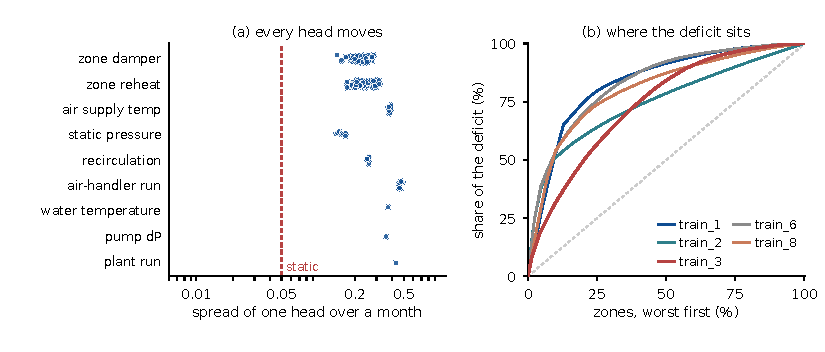
\includegraphics[width=\linewidth]{figures/fig_appendix_behaviour.pdf}
\caption{(a) the spread of each of the 219 heads of the reported checkpoint, median over the months in which that head is active; the dashed line is the threshold below which a head would be called static. (b) the cumulative share of the scored deficit, zones ordered worst first; the diagonal is an even building.}
\label{fig:appendix_behaviour}
\end{figure}

\subsection{The action follows the deficit}

The zones in trouble are not the ones receiving less air or heat. On occupied steps the rank correlation between a zone's mean damper position and its mean deficit is positive on all five buildings, from $+0.16$ to $+0.77$: the further out of band a zone sits, the more air it is given.

Reheat looks inconsistent until the sign of the deficit is taken into account, and then it is coherent. On \texttt{train\_1} and \texttt{train\_8}, where 87\,\% and 80\,\% of the deficit is on the cold side, reheat correlates $+0.49$ and $+0.50$ with the deficit. On \texttt{train\_3} and \texttt{train\_6} the deficit is 80\,\% and 78\,\% on the hot side, and reheat correlates $-0.51$ and $-0.35$: the hot zones get less reheat. \texttt{train\_2}, 68\,\% cold, is the null case at $+0.03$.

The limit of this subsection is the sample. The correlations run across 30 to 85 zones on one pooled set of months, so the intervals are wide and a coefficient near 0.2 is not evidence that the policy cannot aim. What it does show is that the actuators point the right way in the aggregate, so the residual on \texttt{train\_3} is better described as a zone the policy cannot hold than as a zone it is not trying to hold.


\subsection{When the score accrues}

Table~\ref{tab:app_daypart} gives the score per step in each day-part, the values plotted in Figure~\ref{fig:time}b. The bins here keep weekdays and weekends apart; the hourly curve of Figure~\ref{fig:time}a averages every day of the month, weekends included, so its 06:00 value sits below the weekday morning bin of the table. Day 0 of every episode is an empty Sunday, and the policy heats through it: across the five buildings the first 24 hours burn 59, 44, 62, 213 and 294\,kWh of gas, and 57 to 93\% of that falls in the last six hours before comfort starts. That day scores 0.0007 to 0.0020, so the heat is bought at night prices and the bill for it arrives on Monday.

The drift over the 30 days is not uniform. \texttt{train\_3} moves fastest, \texttt{train\_6} and \texttt{train\_2} at a third and a quarter of that rate ($1.1\times10^{-4}$ and $0.9\times10^{-4}$ per day), and \texttt{train\_1} and \texttt{train\_8} are flat at $5.7\times10^{-5}$ and $3.5\times10^{-6}$. The residual therefore grows on the three largest plants and stays put on the two smallest, which is an early warning for the tail rather than a month that comes apart.

\begin{table}[h!]
\centering
\small
\begin{tabular}{@{}lrrrr@{}}
\toprule
day-part & \texttt{PID} & Long & Mid & Final \\
\midrule
weekday night & 0.0037 & 0.0049 & 0.0064 & 0.0045 \\
weekday morning & 0.1280 & 0.0633 & 0.0502 & 0.0459 \\
weekday afternoon & 0.1043 & 0.0585 & 0.0381 & 0.0353 \\
weekday evening & 0.0974 & 0.0616 & 0.0356 & 0.0326 \\
weekend day & 0.0061 & 0.0012 & 0.0002 & 0.0001 \\
weekend night & 0.0061 & 0.0017 & 0.0004 & 0.0003 \\
\bottomrule
\end{tabular}
\vspace{4pt}
\caption{Score per step in each day-part, averaged over the 90 held-out months. A step is five
minutes; the bins are the weekday night (19:00--06:00), morning (06:00--12:00), afternoon
(12:00--16:00) and evening (16:00--19:00), and the weekend day and night.}
\label{tab:app_daypart}
\end{table}

\section{Limitations}
\label{app:limits}

One seed. Every arm in this paper is seed 75, and the two seeds we ran differ by 6\,\%. Differences smaller than that are not resolved here, and the headline result is a single run of the final recipe, not a distribution.

One episode per scenario, and it is deterministic. Each of the 90 months is a single trajectory, so occupancy draws one realisation and the spread we report is across scenarios and months, never across randomness. A building whose sampled occupancy happens to be unusual is not averaged out, and the five worst months of Figure~\ref{fig:appendix_scores} are one draw.

The evaluation set is ours, not the competition's. Five buildings, two windows per trained station and eight for Minneapolis; the leaderboard uses six unseen buildings and five unseen stations. The 90-month mean is the right number for a controlled comparison and it is not a leaderboard estimate. We do not convert one into the other.

The checkpoint was selected on the training panel. The 90 months did not choose the weights, which is the point, but the panel is read while the policy is still changing, so the choice is one decision taken once on a noisy curve (Section~\ref{app:selection}).

The only baseline is the benchmark's controller. We compare against \texttt{pid\_water} as shipped and against three other shipped controllers on the training scenarios, and none of them was tuned for this comparison. A tuned PID, a model-predictive controller or a schedule optimiser would be a stronger test, and the claim we make is correspondingly narrow: better than the controllers the benchmark supplies, not better than classical control.

The comfort term is unbounded and the metric is a mean. One zone can dominate a month and one month can dominate the mean: the five worst months are a single building and carry a fifth of the total. A mean over a designed set of 90 months is a fragile summary, which is why the per-building and per-climate breakdown is reported beside it.

Sim-to-real is untested. Training and scoring both happen inside the benchmark's simulator, which carries the published building models and a stochastic occupancy model but no sensor drift, no stuck damper, no actuator delay and no operator. Whether the behaviour survives a real plant is unknown, and it is the largest open question in the work.

The fine-tuning did not happen at the final scale. The recipe was chosen by 50M-step arms on four scenarios, and the reported run is one 200M-step run on 30 scenarios. The transfer from four to thirty scenarios and from 50M to 200M steps is one observation, not a measured scaling law, and the 30-scenario budget was not swept.

The interface has a fixed envelope. Ninety zone slots, nine air handlers and one plant cover every building in this study; a building outside that envelope, with more than 90 zones or several plants, cannot be written into the layout without changing it, and the submission would have to be rebuilt rather than retrained on the same weights.

What we would test next follows from those limits: a second seed at the final scale, a tuned or model-predictive baseline on the same months, a fault-injected version of the simulator, and a single real zone in a real building. Each of them attacks a limitation above rather than adding a result.

\end{document}
